\documentclass[12pt]{scrartcl}

\input{../styles/Packages}
\input{../styles/FormatAndHeader}

% Zusätzliche Pakete
\usetikzlibrary{arrows.meta, calc, positioning}

\setcounter{sheetnr}{9}   % Übungsblatt 9
\setcounter{exercisecounter}{0}

\begin{document}
    \header

% ==============================================================
%  Aufgabe 9.1: Überdeckungsgraph
% ==============================================================
    \exercise{Abgabe 9.1: \"Uberdeckungsgraph}


    \begin{figure}[htbp]
        \centering
        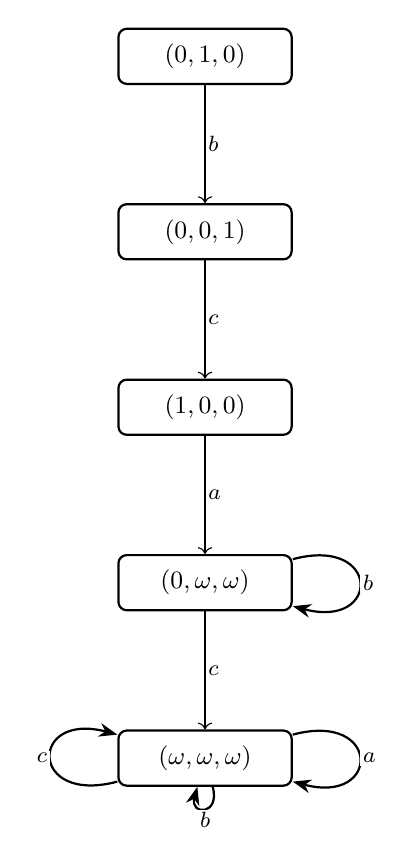
\begin{tikzpicture}[
            node distance=2cm,
            state/.style={rectangle, draw=black, thick, rounded corners=3pt,
            minimum width=2.2cm, minimum height=0.7cm,
            font=\small, align=center},
            every edge/.style={draw, thick, -Stealth},
            lbl/.style={font=\footnotesize, fill=white, inner sep=1pt}
        ]

% ----- Knoten (vertikale Kette) -----
            \node[state] (m0) {$(0,1,0)$};
            \node[state, below=1.5cm of m0] (m1) {$(0,0,1)$};
            \node[state, below=1.5cm of m1] (m2) {$(1,0,0)$};
            \node[state, below=1.5cm of m2] (m3) {$(0,\omega,\omega)$};
            \node[state, below=1.5cm of m3] (m4) {$(\omega,\omega,\omega)$};

% ----- Kanten -----
            \draw[->] (m0) -- node[lbl, right] {$b$} (m1);
            \draw[->] (m1) -- node[lbl, right] {$c$} (m2);
            \draw[->] (m2) -- node[lbl, right] {$a$} (m3);
            \draw[->] (m3) -- node[lbl, right] {$c$} (m4);

% Selbstschleifen
            \draw[->] (m3) edge[loop right, looseness=5] node[lbl, right] {$b$} (m3);
            \draw[->] (m4) edge[loop right, looseness=5] node[lbl, right] {$a$} (m4);
            \draw[->] (m4) edge[loop below, looseness=5] node[lbl, below] {$b$} (m4);
            \draw[->] (m4) edge[loop left, looseness=5] node[lbl, left] {$c$} (m4);

        \end{tikzpicture}
        \caption{\"Uberdeckungsgraph f\"ur das Petrinetz $P_4$}
    \end{figure}


    \newpage

% ==============================================================
%  Aufgabe 9.2: Fallen und Deadlocks
% ==============================================================
    \exercise{Abgabe 9.2: Fallen und Deadlocks}
    \renewcommand{\arraystretch}{1.3}
    \begin{center}
        \begin{tabular}{l|c|c|c|c}
            & Vorbereich & Nachbereich & Falle & Deadlock \\
            \hline
            $\{A\}$           & $\{c\}$       & $\{a\}$       & nein & nein \\
            \hline
            $\{B\}$           & $\{a\}$       & $\{b\}$       & nein & nein \\
            \hline
            $\{C\}$           & $\{a, b\}$    & $\{c\}$       & nein & nein \\
            \hline
            $\{D\}$           & $\{b\}$       & $\{c\}$       & nein & nein \\
            \hline
            $\{A, B\}$        & $\{a, c\}$    & $\{a, b\}$    & nein & nein \\
            \hline
            $\{A, C\}$        & $\{a, b, c\}$ & $\{a, c\}$    & ja   & nein \\
            \hline
            $\{A, D\}$        & $\{b, c\}$    & $\{a, c\}$    & nein & nein \\
            \hline
            $\{B, C\}$        & $\{a, b\}$    & $\{b, c\}$    & nein & nein \\
            \hline
            $\{B, D\}$        & $\{a, b\}$    & $\{b, c\}$    & nein & nein \\
            \hline
            $\{C, D\}$        & $\{a, b\}$    & $\{c\}$       & nein & nein \\
            \hline
            $\{A, B, C\}$     & $\{a, b, c\}$ & $\{a, b, c\}$ & ja   & ja   \\
            \hline
            $\{A, B, D\}$     & $\{a, b, c\}$ & $\{a, b, c\}$ & ja   & ja   \\
            \hline
            $\{A, C, D\}$     & $\{a, b, c\}$ & $\{a, c\}$    & ja   & nein \\
            \hline
            $\{B, C, D\}$     & $\{a, b\}$    & $\{b, c\}$    & nein & nein \\
            \hline
            $\{A, B, C, D\}$  & $\{a, b, c\}$ & $\{a, b, c\}$ & ja   & ja   \\
        \end{tabular}
    \end{center}

\end{document}
